\subsubsection{Application Survey}
The current main developer of new features is Johannes Wolf. 
He is supported by Johannes Linke who is mainly responsible for a good coding style, including code review and refactoring. 
We interview them about information regarding the first steps of our project.

\paragraph{Development Paradigm and Development Languages}
There are no development paradigms explicitly determined.
But as stated there is a main developer responsible for code review.
As it is, all newly developed code is reviewed before it is accepted.
Everyone is able to review code and discuss it with the author and other reviewers.
This practice shall ensure readable code and distribute knowledge about code changes.
Additionally, it is implicitely assumed that paradigms of the used development languages are followed.
The development languages are:
\begin{itemize}
    \item Python 3 through the Django framework
    \item HTML
    \item Javascript
    \item CSS
\end{itemize}
As an example for paradigms given by the languages we checked the document known as \emph{PEP 0008}%
\footnote{\url{https://www.python.org/dev/peps/pep-0008/}}.
This is the style guide for Python code written by Guido van Rossum, the author of Python, and followed by most open source projects in Python.

\paragraph{Requirements / Specification / Documentation / Artefacts}
Requirements were elaborated at the start of EvaP's predecessor EvaJ several years ago.
No original artifacts were stored even though most requirements still hold. 
Examples are:
\begin{itemize}
    \item Evaluation should be anonymous
    \item Written feedback is only readable by a small, strongly specified selection of people
    \item Written feedback is reviewed before it is available to the lecturer
\end{itemize}
Symptomatic for an open source project managed by students there is no formal specification of EvaP. 
Though there are different information gathered in the project wiki hosted on Github%
\footnote{\url{https://github.com/fsr-itse/EvaP/wiki}}.
The responsibility to specify new features is on the main developer, Johannes Wolf.
He collaborates directly with the users of the feature.
%TODO EvaP FAQ


\paragraph{Current testing status / Bug repositories}
The project is hosted open source on GitHub.
Different tools allow to include badges on the overview page to display the status of the latest build (\autoref{fig:testing-tools}).
The following tools are already used:
\begin{itemize}
    \item \emph{Travis CI}: 
    A continuous integration service to build and test projects hosted on GitHub
    \item \emph{Gemnasium}:
     An automated service for monitoring project dependencies for possible updates
     \item \emph{Landscape}:
     A service checking the code for errors, code smells and deviations from stylistic conventions
     \item  \emph{Coveralls}:
     A service relying on Travis CI that tracks the code coverage
     \item 
     Another feature of Github is used to track bugs: the label \emph{[T] Bug} for \emph{issues}.
\end{itemize}
These tools are already the most common used ones for open source python development for good reasons, as they provide a good feature set at no costs.
Therefore we will not research further tools for bug tracking, source code versioning or automated testing.
\begin{figure}[h]
    \centering
    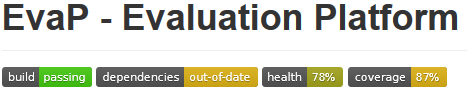
\includegraphics[width=0.5\textwidth, keepaspectratio]{graphics/testing-tools-github}
    \caption{Badges of testing tools on the GitHub overview page (01.12.2015)}
    \label{fig:testing-tools}
\end{figure}


\paragraph{Personal involvement}
Our first contact with EvaP was as users. 
As HPI bachelor students we evaluated courses of the first semester.
As a tutor for a course Stefan used EvaP to read feedback.
As a member of the student representatives Jennifer reviewed comments before publishing the evaluation.
During the \emph{Evap Hackday 2014} and \emph{Evap Hackday 2015} Jennifer joined the team of developers.
She familiarized herself with the development practice to fork, code and create pull requests for review and solved several small issues.
